%%%%%%%%%%%%%%%%%%%%%%
\section{Evaluation}
%%%%%%%%%%%%%%%%%%%%%%

In this section, we profile various aspects of our PIFO design to justify our design choices and demonstrate its capability to achieve line rate performance. We use a  200MHz reference clock in these evaluations to target the NetFPGA-SUME card.

\subsection{Priority Queue Evaluation}

As explained in Section~\ref{sec:priority-queue}, the priority queue consists of a single skip list and a cache. It is designed to satisfy two properties:
\begin{enumerate}
  \item Packet descriptors can be enqueued at less than line rate
  \item Packet descriptors can be dequeued from the head at line rate
\end{enumerate}

The following sections describe experiments that allow us to characterize the enqueue and dequeue performance of a single priority queue.

\subsubsection*{Effect of Fill Level}
Descriptors can be enqueued into the cache every other clock cycle. The main factor that drives the rate at which descriptors can be enqueued into the skip list is the number of memory operations that are required to find the appropriate insertion location, which increases logarithmically with the number of the descriptors in the skip list. We define the fill level as the number of descriptors in both the skip list and the cache.

Figure \ref{fig:fill_level} shows the effect of the fill level on both the enqueue and the dequeue latency, that is, the number of clock cycles required to complete each of these operations. This experiment uses a skip list with a capacity of 2048 elements (using 12 levels) and 16-entry cache. Each average and maximum is computed over 100 samples. As expected, the enqueue latency increases logarithmically with the number of descriptors and the maximum possible enqueue latency is 130 clock cycles, which agrees with the theoretical maximum given by equation \ref{worst-case-insert_eqn}, with $L = 12$, $T_{Rd}$ = 2, $T_{Wr}$ = 1, $K_{1}$ = 3, and $K_{2}$ = 7.

This result constrains two additional aspects of the design:
\begin{enumerate}
  \item The minimum size of the register-based cache to ensure that it has enough capacity to avoid running empty during the longest possible enqueue operation into the skip list.
    \item The number of priority queues that must be used in parallel in order to support enqueue operations at line rate.
\end{enumerate}

All packets used in this experiment are 64B in length, which take 2 cycles to transfer using our 32B data-path. The dequeue latency plot shows that these 64B packets can be removed in three to five cycles depending on whether the dequeue operation is directly preceded by an insertion into the register cache. This is more than fast enough to meet our 13.44 cycle deadline for 10Gb/s operation.

\begin{figure}[!h]
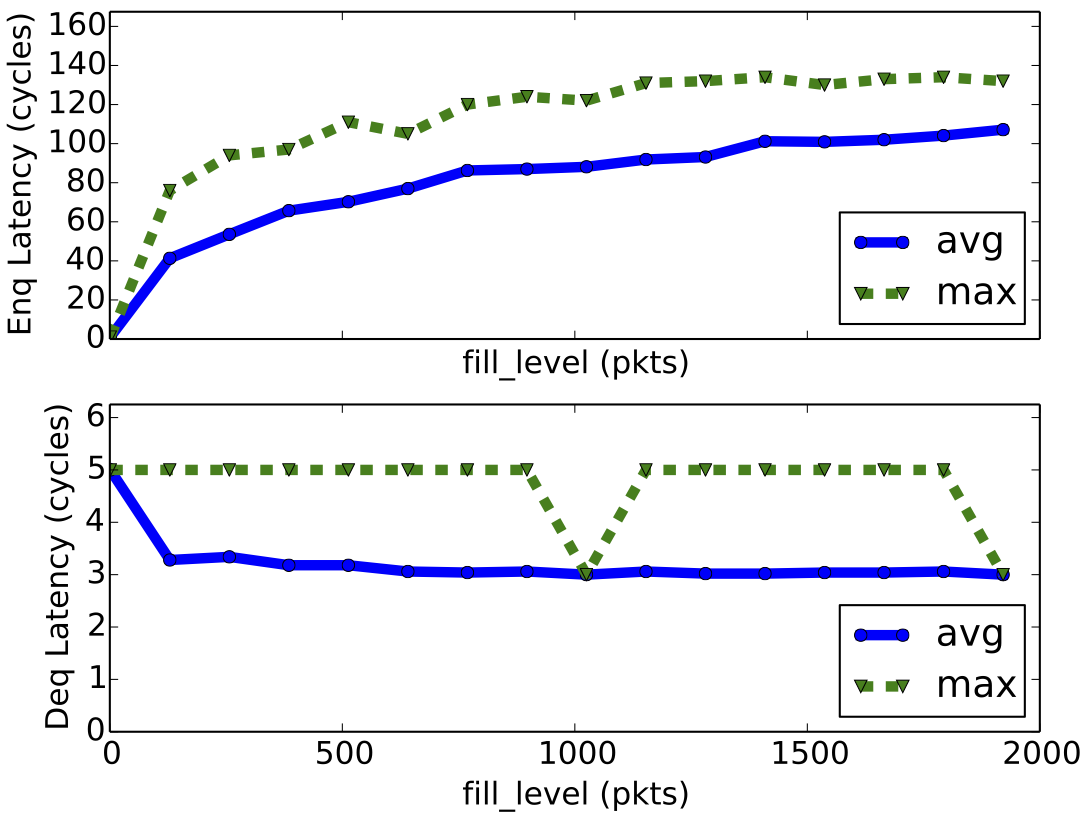
\includegraphics[width=1\linewidth]{figures/eval/enq_deq_v_fill_level}
\caption{Effect on the enqueue and dequeue latencies when the number of entries in the priority queue increases.}
\label{fig:fill_level}
\end{figure}

\subsubsection*{Sizing the Register-based Cache}
The cache must be large enough to satisfy two constraints:
\begin{enumerate}
  \item Large enough to absorb the variations in the rate at which it is being filled by the background process that is replenishing it with descriptors from the skip list.
  \item Large enough to be able to hold enough descriptors such that it will not run empty when the longest possible skip list insertion begins and replenishment from the skip list temporarily stops.
\end{enumerate}

Both of these conditions must be met in order to guarantee that the scheduler will remain work conserving under all conditions. 

To satisfy the first constraint, we must be able to bound the rate at which descriptors are dequeued from the skip list and inserted into the cache. Fortunately, the deterministic structure of the skip list allows us to do exactly that. The maximum number of clock cycles required to dequeue an element from the head of the skip list is directly related to the number of levels in which the head element is present ($L$). This relationship is given by the following expression,

\begin{equation}\label{worst-case-remove_eqn}
T_{Rd} \times L + K_{3}
\end{equation}
where:\\
\indent $T_{Rd}$ = node read time\footnote{Writes are performed as well but they do not contribute to the latency because they are performed in parallel with the reads} = 2 clock cycles\\
\indent $K_{3}$ = processing overhead = 6 clock cycles\\

The deterministic skip list structure property enforces that the node heights, i.e. the number of levels in which they appear, are well distributed. This means that the dequeue rate from the skip list is mostly constant. Figure \ref{fig:cache_fill} shows the fill level of the cache during an experiment where the skip list starts out filled with 2K descriptors and is then drained at a rate of one descriptor every 12 cycles, i.e., faster than line rate. We see that the number of descriptors in the cache never drops by more than two indicating that it is indeed being filled faster than it is being drained. Our measurements indicate that on average, the head element can be removed from the skip list in 8 clock cycles and in the worst case it can take up to 30 clock cycles, just over two minimum packet times.

\begin{figure}[!ht]
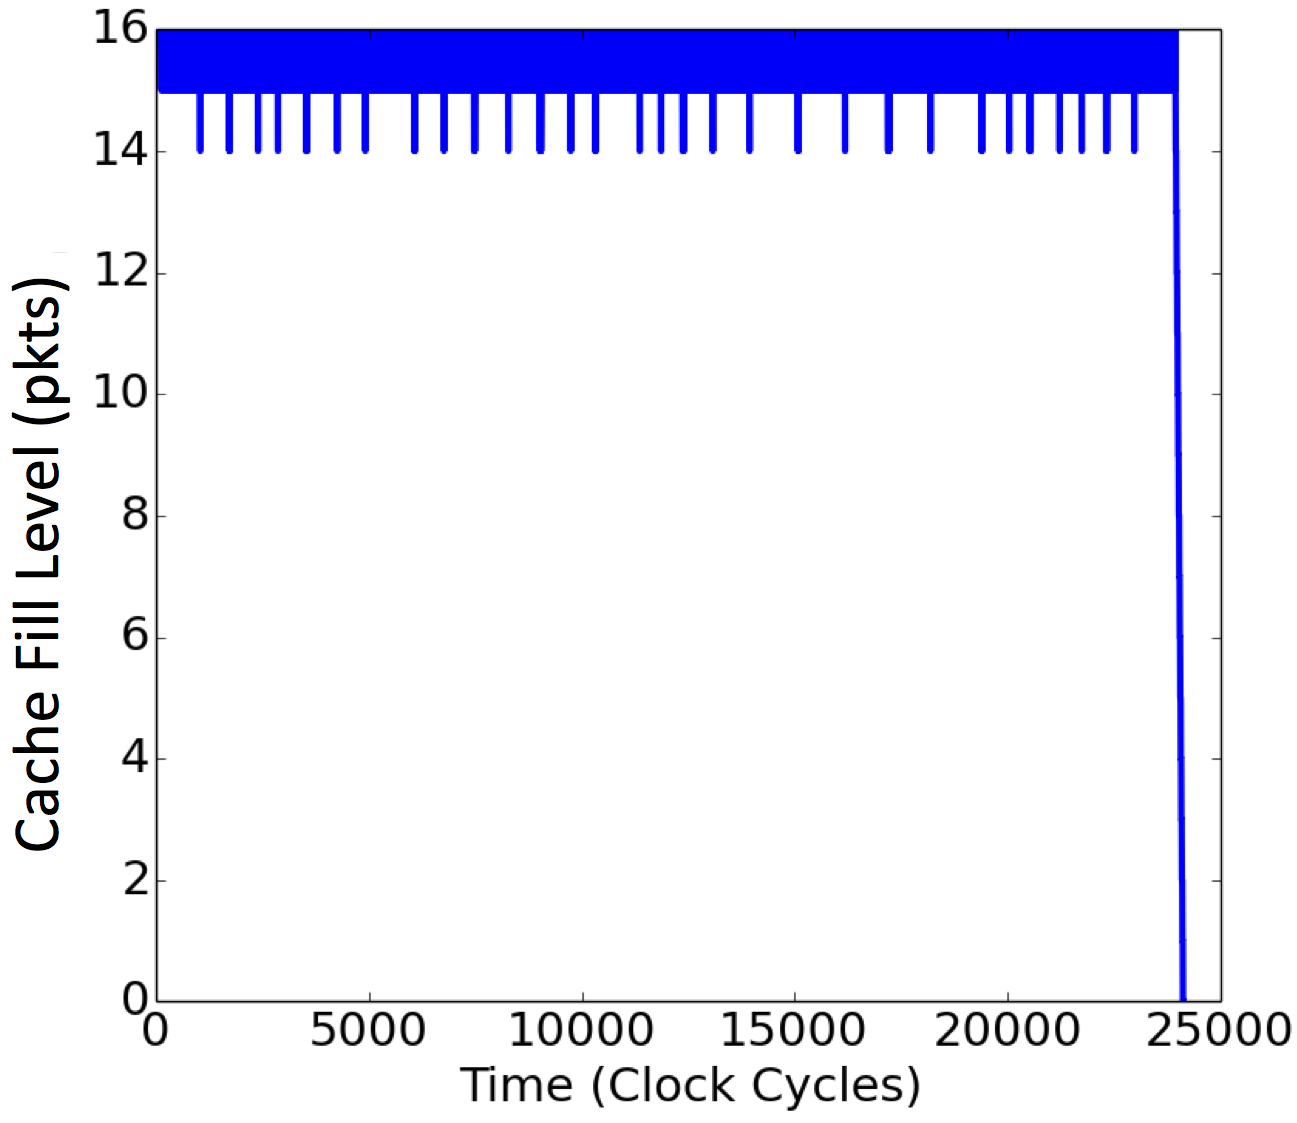
\includegraphics[width=1\linewidth]{figures/eval/cache_fill_plot}
\caption{The fill level of the cache while draining a skip list with 2K descriptors.}
\label{fig:cache_fill}
\end{figure}

The cache must also be large enough to avoid going empty during a long skip list enqueue operation. This turns out to be a tighter constraint than (1) because an enqueue into the skip list can last up to 130 cycles (with a fill level of 2000 descriptors). The output register will be drained at line rate of up to one descriptor every 13.44 cycles. This means than it must be able to hold at least 10 descriptors in order to sustain line rate without missing any deadlines.

\subsection{PIFO Evaluation}

A single priority queue cannot support enqueue operations at line rate. This is why a PIFO is composed of multiple priority queues combined in parallel and the enqueue operations are load balanced across all of them. The following section describes the results of the experiment we used to analyze the relationship between the enqueue latency and the number of parallel priority queues.

\subsubsection*{Number of parallel priority queues}
We conducted multiple experiments varying the number of parallel priority queues and use a fill level of 2000 packets. We report the average and maximum enqueue latency over 100 samples for each experiment. Figure \ref{fig:num_skip_lists} shows that the average enqueue latency is very sensitive to the number of priority queues that are used in parallel. As the number of priority queues increases, the fill level of each one decreases and hence enqueue operations complete more quickly. This results in an inverse log relationship between enqueue latency and number of priority queues. We find that the design must use at least 12 parallel skip lists to support line rate enqueue operations, that is, one enqueue every 13.44 cycles. Figure \ref{fig:num_skip_lists} also shows that the dequeue latency is well under this 13.44 cycle requirement as well.

\begin{figure}[!h]
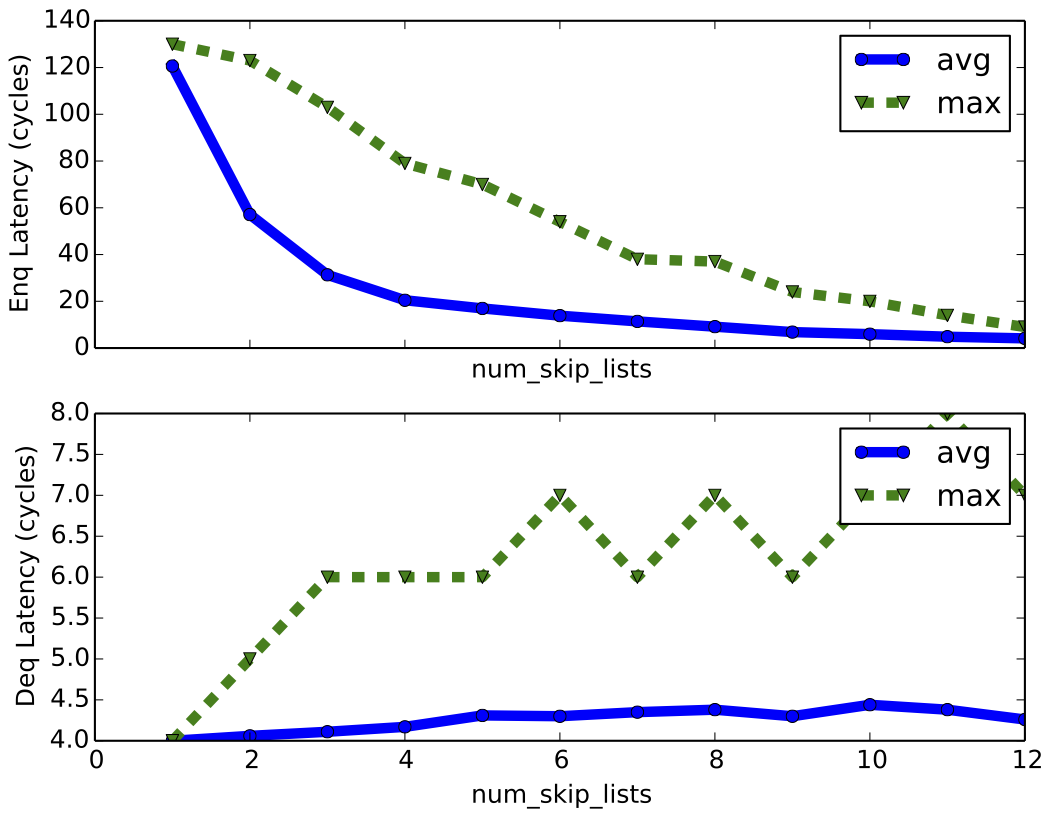
\includegraphics[width=1\linewidth]{figures/eval/enq_deq_v_num_skip_lists}
\caption{Effect of the number of parallel priority queues on the overall enqueue and dequeue latencies}
\label{fig:num_skip_lists}
\end{figure}



